\section{Προσαρμοσμένη Μάθηση}
\subsection{Μαθηματικός Ορισμός Μοντέλου Μάθησης}
Το \textlatin{ChronoQuest} θα έχει ένα σύστημα προσαρμοσμένης μάθησης. Η αρμοδιότητά του θα είναι η πιθανοτική αξιολόγηση με βάση τέσσερις παραμέτρους \cite{bkt_wiki}:
\begin{itemize}
    \item \textbf{$p_{init}(s)$}: Η πιθανότητα ο χρήστης να έχει γνώση πάνω σε κάποιο θέμα/ενότητα \textbf{$s$}.
    \item \textbf{$p_{learn}(s)$}: Η πιθανότητα ο χρήστης να μάθει το θέμα $s$ μετά από προσπάθεια
    \item \textbf{$p_{slip}(s)$}: Η πιθανότητα ο χρήστης να κάνει λάθος παρόλο τη γνώση του στο θέμα $s$
    \item \textbf{$p_{guess}(s)$}: Η πιθανότητα ο χρήστης να απαντήσει σωστά παρόλο τη έλλειψη γνώσης του στο συγκεκριμένο θέμα $s$
\end{itemize}

Οι παραπάνω παράμετροι είναι μέρος του αλγόριθμου γνωστού ως \textlatin{\textbf{Bayesian Knowledge Tracing (BKT)}}. Αυτός ο αλγόριθμος, με τη χρήση των τεσσάρων παραμέτρων, μας δίνει μια \textbf{πιθανότητα επιδεξιότητας} ενός χρήστη $u$ για ενα συγκεκριμένη θέμα $s$. Οι παρακάτω εξισώσεις μπορούν να εφαρμοστούν για την ενημέρωση του μοντέλου όταν αλληλεπιδρά ο χρήστης $u$:

(1) Αρχικοποίηση:
$$p(X_1, s, u) = p_{init}$$

(2) Υπό συνθήκη πιθανότητα όταν ο χρήστης απαντάει σωστά:
$$p(X_t\ |\ obs = correct, s, u) = \frac{p(X_t, s, u) \cdot (1 - p_{slip}(s))}{p(X_t,s,u) \cdot (1 - p_{slip}(s)) + (1 - p(X_t, s, u)) \cdot p_{guess}(s) }$$

(3) Υπό συνθήκη πιθανότητα όταν ο χρήστης απαντάει λάθος:
$$p (X_t\ |\ obs = wrong, s, u) = \frac{p(X_t, s, u) \cdot p_{slip}(s)}{p(X_t,s,u) \cdot p_{slip}(s) + (1 - p(X_t, s, u)) \cdot (1 - p_{guess}(s)) }$$

(4) Ενημέρωση της πιθανότητας επιδεξιότητας:
$$p(X_{t+1}, s, u) = p(X_t\ |\ obs, s, u) + (1 - p(X_t\ |\ obs, s, u)) \cdot p_{learn}(s)$$

(5) Πιθανότητα ο χρήστης να κατέχει την έννοια σε επόμενη αλληλεπίδραση:
$$p(C_{t+1}, s, u) = p(X_{t+1}, s, u) \cdot (1 - p_{slip}(s)) + (1 - p(X_{t+1}, s, u)) \cdot p_{guess}(s)$$

Το σύστημα προσαρμοσμένης μάθησης θα παίρνει αποφάσεις για ένα χρήστη με βάση την εξίσωση (5).

\subsection{Χρήση εντός του \textlatin{ChronoQuest}}

Το σύστημα \textlatin{BKT} που ορίστηκε παραπάνω, θα χρησιμοποιηθεί για την πρόβλεψη και την καταγραφή της απόδοσης του χρήστη στα διάφορα θέματα.

Ένα θέμα μπορεί να είναι η γεωγραφία του τόπου, ή η ιστορία του. Έτσι, η απόδοση του χρήστη θα αξιολογείται με βάσει αυτά τα θέματα. 

\subsection{Αλγόριθμος Υπολογισμού Απόδοσης}
Αν αποθηκεύσουμε κάθε πιθανότητα επιδεξιότητας που καταγράφεται του μοντέλου \textlatin{BKT} μπορούμε να κατασκευάσουμε ένα ιστορικό επιδεξιότητας ή καλύτερα μια \textbf{καμπύλη μάθησης} του χρήστη για ένα θέμα.

\begin{figure}[H]
    \centering
    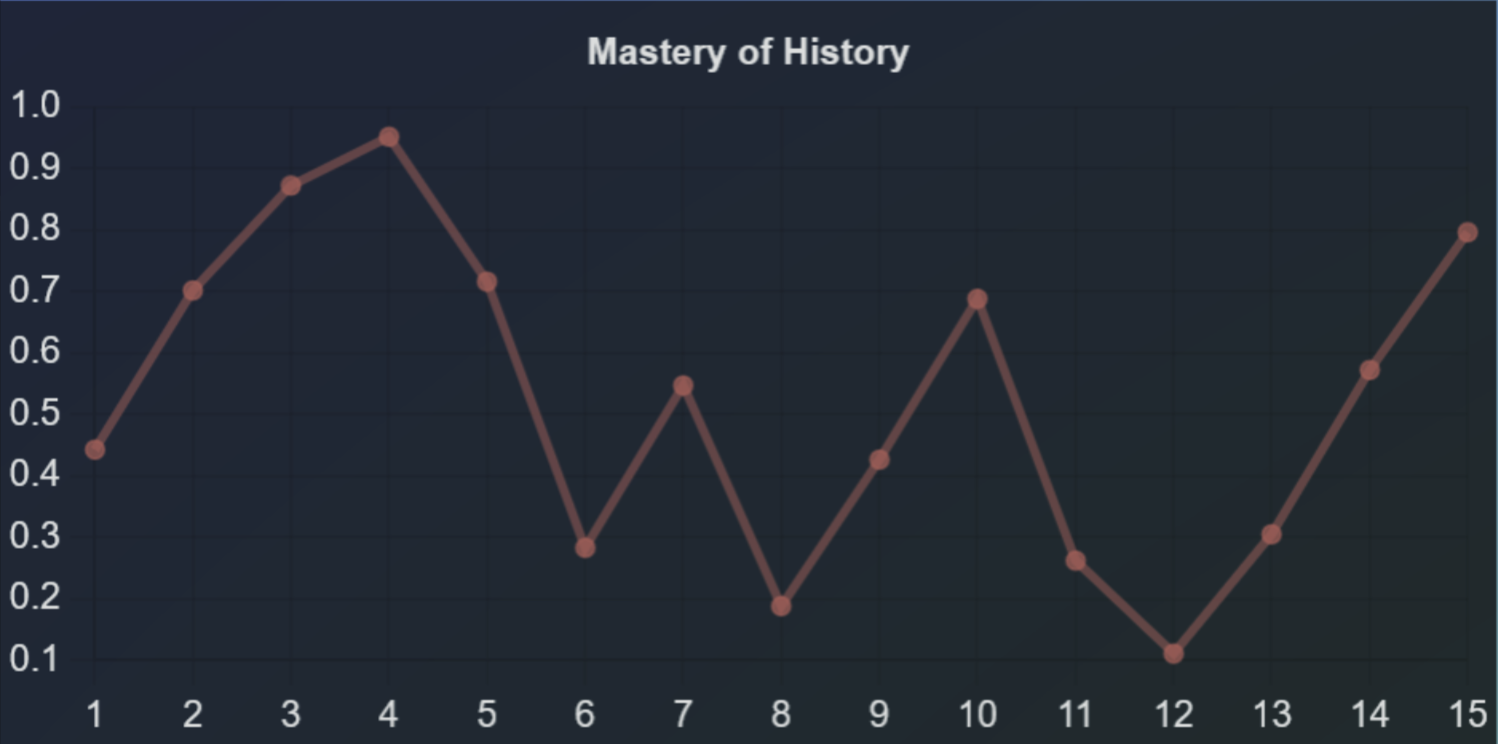
\includegraphics[width=0.5\linewidth]{img/MasteryGraph.png}
    \caption{Καμπύλη Μάθησης στη πράξη}
\end{figure}

Ένας άνθρωπος μπορεί οπτικά μέσω του παραπάνω γραφήματος να βγάλει σωστά συμπεράσματα για την απόδοση του. Ας δούμε πως μπορούμε να "μαθηματικοποιήσουμε" την διαδικασία λήψης συμπερασμάτων. Προτού δούμε τη κάθε μετρική, ας ορίσουμε κάποια μαθηματικά σύμβολα:

\begin{align*}
    s(t):\ &\text{Η επιδεξιότητα του χρήστη τη χρονική στιγμή}\ t  
\end{align*}

Θα χρησιμοποιήσουμε 4 μετρικές για να αποκτήσουμε μια πολύ καλή εικόνα της απόδοσης του χρήστη:
\subsubsection{Ταχύτητα Μάθησης}
Ασχολείται με το ρυθμό αλλαγής της καμπύλης μάθησης -- για τους μαθηματικούς: με τη παράγωγο της καμπύλης. Η μετρική αυτή μας δίνει τρείς αριθμούς:

\begin{align*}
    v_{current}(t) &= s(t) - s(t - 1) \\
    v_{average} &= \frac{\sum_{t = 1}^{n}{s(t)}}{n} \\
    v_{acceleration}(t) &= 
    \begin{cases}
        0, & \text{αν } t < 2 \textlatin{ ή } t S_{x^2} - (S_x)^2 \leq 10^{-10} \\
        \displaystyle\frac{t S_{xt} - S_x S_t}{t S_{x^2} - (S_x)^2}, & \text{αλλιώς}
    \end{cases}
\end{align*}

Ο τρίτος τύπος -- η επιτάχυνση, είναι η παράγωγος του της γραμμικής παλινδρόμης (\textlatin{Linear Regression Slope}) της ανέξάρτητης μεταβλήτης $t$ σε σχέση με την εξαρτημένη μεταβλητή $x$ που εδώ θεωρείται ότι $x = 0, 1, 2, ...$. Τα σύμβολα στο τύπο της επιτάχυνσης αναλύονται περαιτέρω:

\begin{align*}
S_x &= \sum_{i=0}^{n-1} x_i = \frac{n(n - 1)}{2} \\
S_t &= \sum_{i=0}^{n-1} t_i \\
S_{xt} &= \sum_{i=0}^{n-1} x_i t_i \\
S_{x^2} &= \sum_{i=0}^{n-1} x_i^2 = \frac{n(n - 1)(2n - 1)}{6}
\end{align*}

Η ταχύτητα μάθησης θα χρησιμοποιηθεί για την απόφαση τις \textbf{προόδου μάθησης} του χρήστη.

\subsubsection{Μοτίβα Απόκρισης}
Τα μοτίβα απόκρισης αναλύουν τη "συμπεριφορά" του χρήστη. Εδώ ορίζονται η εξής μετρικές:
\begin{itemize}
    \item \textbf{Ομαδοποιήση Λαθών (\textlatin{Error Clustering})}: Μια απλή στατιστική προσέγγιση για την ποσοτικοποίηση συσταδοποίησης λαθών. Η τιμή που μας δίνει αυτη η μετρική αν είναι \textbf{χαμηλή} σημαίνει ότι ο χρήστης κάνει λάθη με σταθερό ρυθμό -- φαινόμενο φυσιολογικό. Αν είναι η τιμή υψηλή, ο χρήστης πολλά λάθη σε κάποια σημεία και λίγα σε κάποια άλλα. Στη περιπτωσή μας, αν εντοπίσουμε υψηλή τιμή συσταδοποίησης, τότε μπορούμε να αυξήσουμε το πόσο σιγουρότητάς μας ότι ο χρήστης κάνει μαντεψίες, καθώς η σείρα των ερωτήσεων δεν ακολουθεί τη σείρα των παραγράφων της θεωρίας. Εν κατακλείδι, όσο πιο ψηλή είναι η τιμή συσταδοποίησης τόσο πιο πολύ θα χαμηλώνει το ολικό σκορ. 
    
    Η ομαδοποίηση λαθών ορίζεται ως εξής:
    $\text{Θεωρούμε:}$
    \begin{align*}
        n:\ &\text{Συνολικός αριθμός απαντήσεων} \\
        w:\ &\text{Το μέγεθος του "παραθύρου"} \\
        r(t) \in {0, 1}:\ &\text{Η ένδειξη σωστής/λάθος απάντησης.}\ 1 = \text{σωστή},\ 0 = \text{λάθος}. 
    \end{align*}

    $$
        d(i) = \frac{1}{w} \sum_{t=i}^{i+w-1}{(1 - r(t))},\ i = 0,1,...,n - w + 1
    $$
    Όπου $d(i)$ είναι η \textbf{τοπική πυκνότητα λαθών} του $i$-οστού "παραθύρου".
    Η τελική τιμή συσταδοποίησης είναι η \textbf{διακύμανση} των τοπικών πυκνοτήτων:

    $$
        C = Var(d)
    $$
    
    \item \textbf{Σταθερότητα (\textlatin{Stability})}: Έχει παρομοιο σκόπο με την ομαδοποίηση, ορίζεται ως εξής:
    \begin{align*}
        a_i &= \frac{1}{w}\sum_{t=i}^{i+w-1} r(t), & i &= 0,\dots,M-1, \\
        \bar a &= \frac{1}{M}\sum_{i=0}^{M-1} a_i, \\
        \sigma &= \sqrt{\frac{1}{M}\sum_{i=0}^{M-1} (a_i - \bar a^2)}, \\
        \mathrm{cv} &= \frac{\sigma}{\bar a}, \\
        S &= 
        \begin{cases}
            1, 
            & \text{αν}\ N < w\ \text{ή}\ M \le 1\ \text{ή}\ \bar a = 0, \\
            \dfrac{1}{1 + \mathrm{cv}}, 
            & \text{αλλιώς}
        \end{cases} 
    \end{align*} 

    Όπου:
    \begin{itemize}
        \item $a_i$: Η \textbf{τοπική ακρίβεια} για το $i$-οστό "παράθυρο".
        \item $\bar a$: Η μέση τιμή των τοπικών ακριβειών.
        \item $\sigma$: Η τυπική απόκλιση των τοπικών ακριβειών.
        \item $cv$: Ο συντελεστής διακύμανσης των τοπικών ακριβειών. 
        \item $S$: Η σταθερότητα του χρήστη δομένου τις απαντήσεις του.
    \end{itemize}
\end{itemize}

Αυτές οι μετρικές θα χρησιμοποιηθούν για τη λήψη αποφάσεων σχετικά με την έκδοση του επαναληπτικού υλικό και του διαγωνίσματος ανα χρήστη.

\subsubsection{Αποδοτικότητα}
Είναι μετρική που μετράει το ρυθμό αύξησης της επιδεξιότητας του χρήστη σχετικά με μια \textbf{ιδανική καμπύλη μάθησης}. Για τους σκοπούς του \textlatin{ChronoQuest}, όριζουμε την ιδανική καμπύλη ως:

$$
    m(n, \alpha) = 1 - e^{n/\alpha}
$$

Όπου:
\begin{itemize}
    \item $n$: Ο αριθμός απαντήσεων/προσπαθειών του χρήστη
    \item $\alpha$: Ο προβλεπόμενος αριθμός που απαιτήται για να φτάσει ο χρήστης στο περίπου 63\% επιδεξιότητα.
\end{itemize}

Θεωρούμε $\alpha = 10$. Η ιδανική καμπύλη μάθησης φαίνεται ως εξής:
\begin{figure}[H]
    \centering
    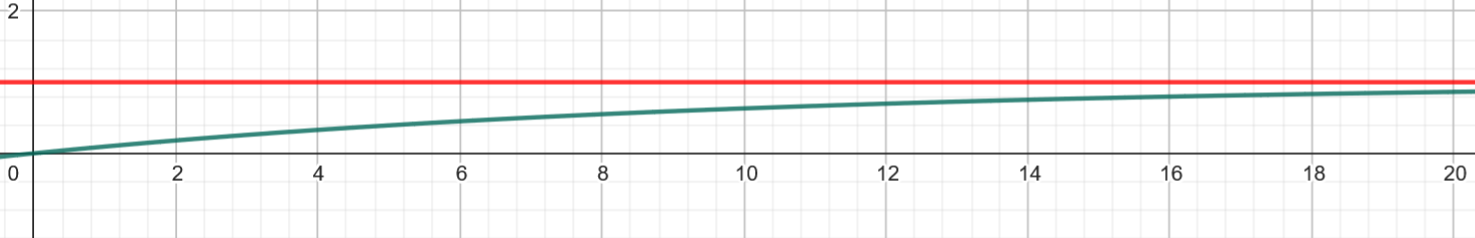
\includegraphics[width=1\linewidth]{img/LearningCurve.png}
    \caption{Ιδανική καμπύλη επιδεξιότητας $m(n, 10)$}
\end{figure}

Για να συγκρίνουμε την απόδοση του χρήστη σχετικά με το ιδανικό μοντέλο, παίρνουμε το ιστορικό επιδεξιότητας $s(t)$ του χρήστη και υπολογίζουμε:
$$
    E = \frac{s(n)}{m(n, 10)}
$$

Βάσει της τιμής της αποδοτικότητας $E$ μπορούμε να βγάλουμε συμπεράσματα:
\begin{itemize}
    \item Αν $E > 1$, ο χρήστης προοδεύει πιο γρήγορα απο τις προβλέψεις του μοντέλου.
    \item Αν $E = 1$, η επιδεξιότητα του χρήστη είναι ακριβώς στο προβλεπόμενο σημείο.
    \item Αν $E < 1$, ο χρήστης προοδεύει πιο αργά απο τις προβλέψεις του μοντέλου.
\end{itemize}

\subsubsection{Πρόοδος Μάθησης}
Αυτη η μετρική συνδυάζει την \textbf{ταχύτητα μάθησης} και τη τωρινή επιδεξιότητα του χρήστη για να βγάλει συμπέρασμα ως προς την "κατάσταση μάθησης" του χρήστη.

Πιο συγκεκριμένα, συνδυάζει τις εξής μετρικές:
\begin{itemize}
    \item Το τωρινό ρυθμό μάθησης \textbf{$v_{current}$}
    \item Την επιτάχυνση μάθησης \textbf{$v_{acceleration}$}
    \item Την τωρινή επιδεξιότητα \textbf{$s(n)$}
\end{itemize}

Με ένα δένδρο αποφάσεων (\textlatin{Decision Tree}), η μετρική μπορεί να καταλήξει στις εξής κατηγορίες:
\begin{enumerate}
    \item \textlatin{Initial}: Η αρχική κατάσταση, σε περίπτωση έλλειπων δεδομένων
    \item \textlatin{Struggling}: Ο χρήστης δυσκολεύεται να ανταποδόσει.
    \item \textlatin{Struggling but Improving}: Ο χρήστης δυσκολεύεται, αλλα δείχνει σημάδια βελτίωσης
    \item \textlatin{Active Learning}: Ο χρήστης βρίσκεται σε ρυθμούς ανάπτυξης.
    \item \textlatin{Steady}: Ο χρήστης
    \item \textlatin{Plateau}
    \item \textlatin{Mastering}
    \item \textlatin{Mastered}
\end{enumerate}